\chapter{Appendix 1: synchronization}

Here are shown the phases oscillations corresponding to fig.\ref{fig:static_sync}-\ref{fig:active_phase_wave}:


\newcommand{\imagewidtha}{0.5\textwidth}


\begin{figure}[h]
 \centering
    \begin{minipage}{\textwidth}
        \centering
        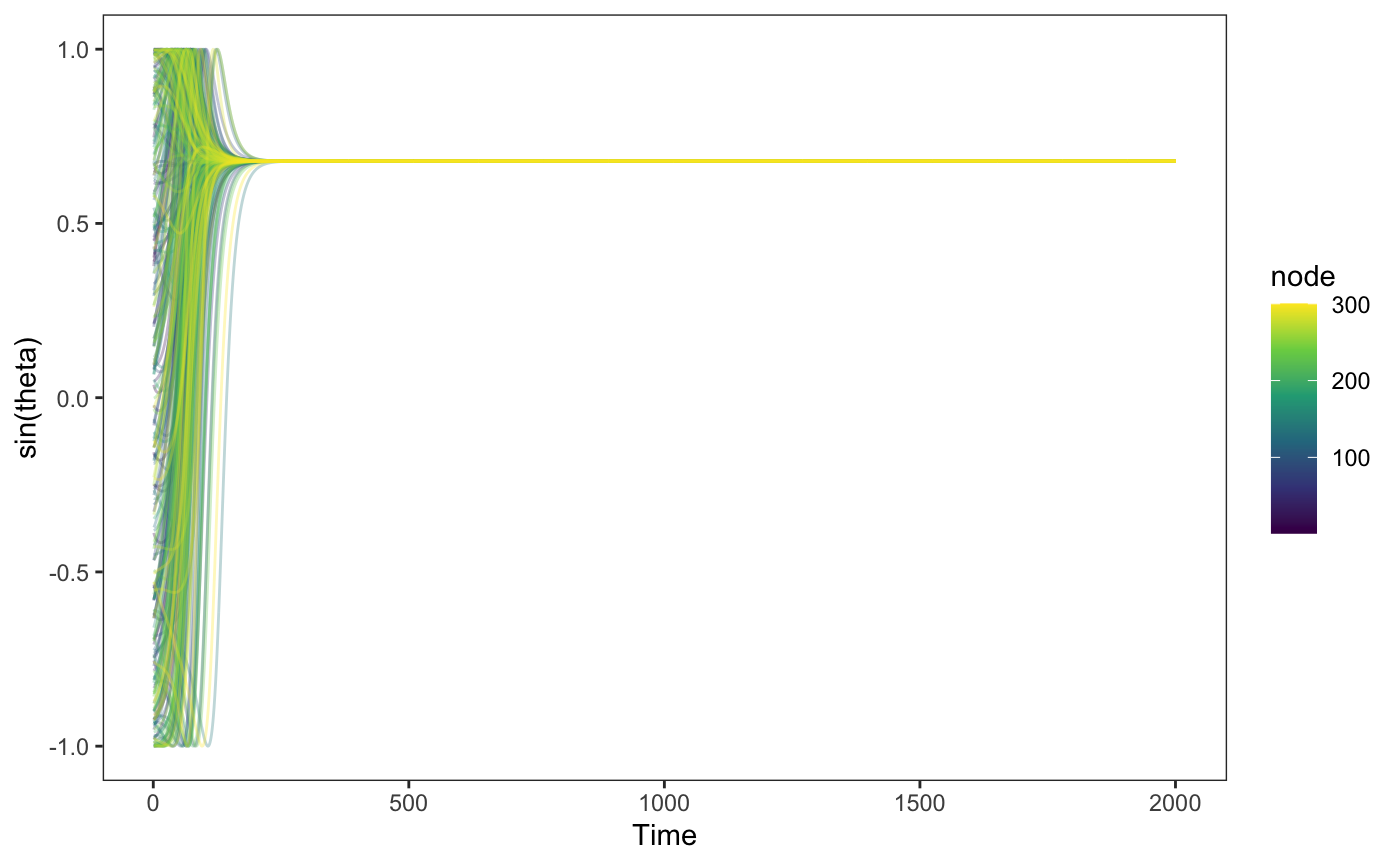
\includegraphics[width=\textwidth]{images/appendix-task1/static_sync.png}
        \caption{Static synchronous state \newline ($K=1$, $J=0.1$)}
        \label{fig:static_sync_p}
    \end{minipage}
\end{figure}

\begin{figure}[h]
 \begin{minipage}{\textwidth}
        \centering
        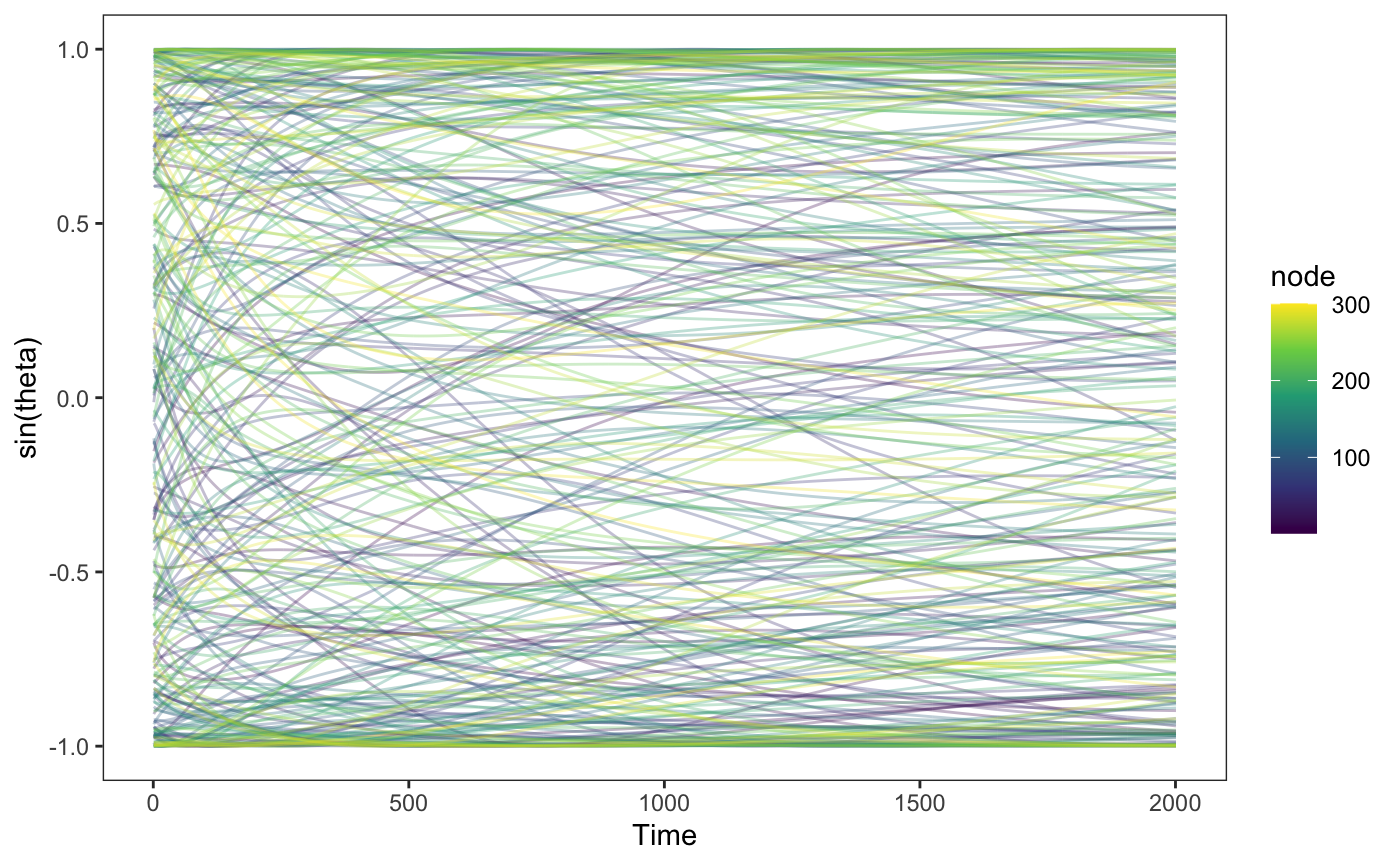
\includegraphics[width=\textwidth]{images/appendix-task1/static_async.png}
        \caption{Static asynchronous state \newline ($K=-1$, $J=0.1$)}
        \label{fig:static_async_p}
    \end{minipage}
\end{figure}

%#########################
\begin{figure}[p]
 \centering
    \begin{minipage}{\textwidth}
        \centering
        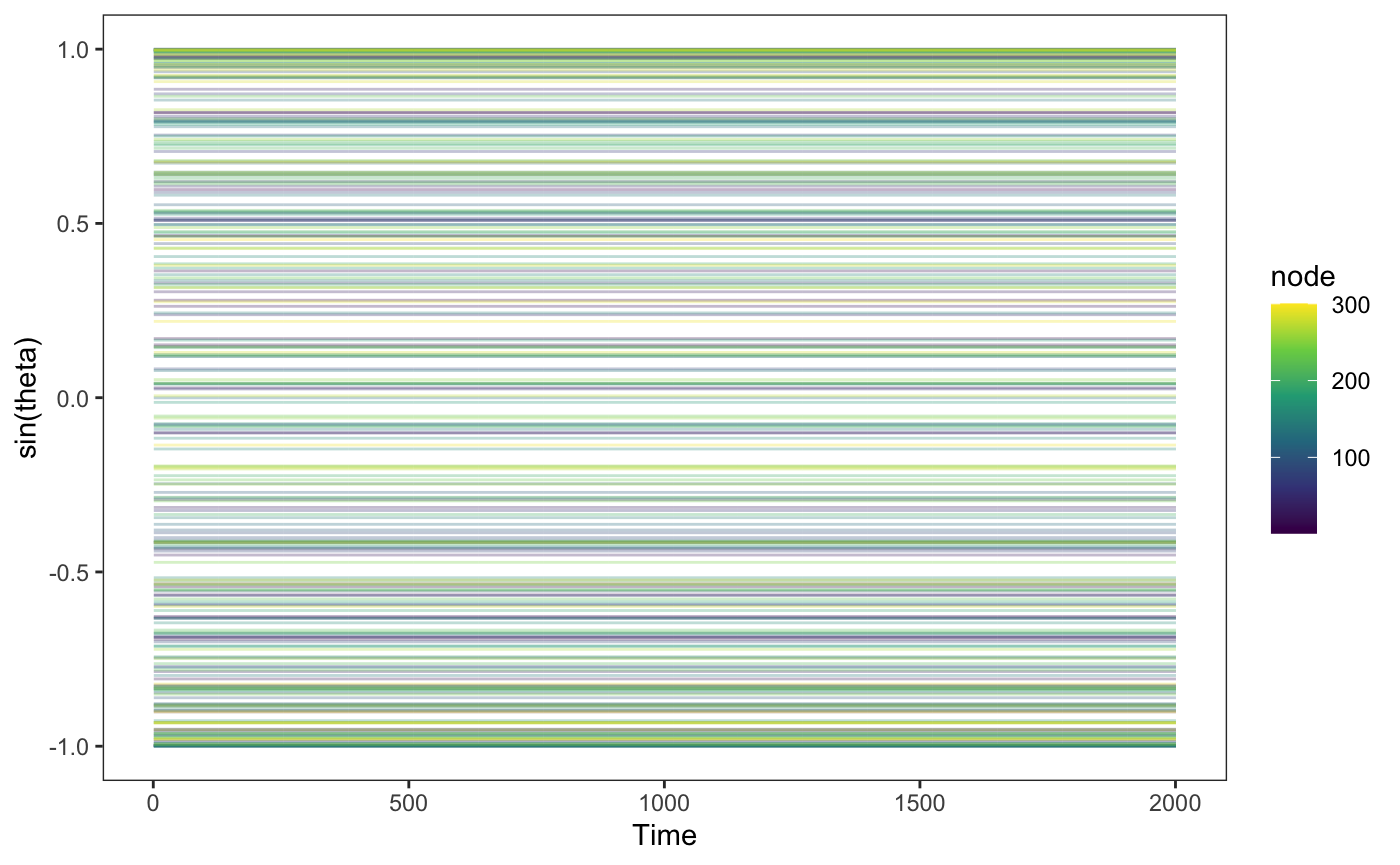
\includegraphics[width=\textwidth]{images/appendix-task1/static_phase_wave.png}
    \caption{Static phase wave state\\ \parbox[t]{\textwidth}{\raggedright ($K=0$, $J=1$)}}
    \label{fig:static_phase_wave_p}
    \end{minipage}
\end{figure}

\begin{figure}[p]
 \begin{minipage}{\textwidth}
        \centering
         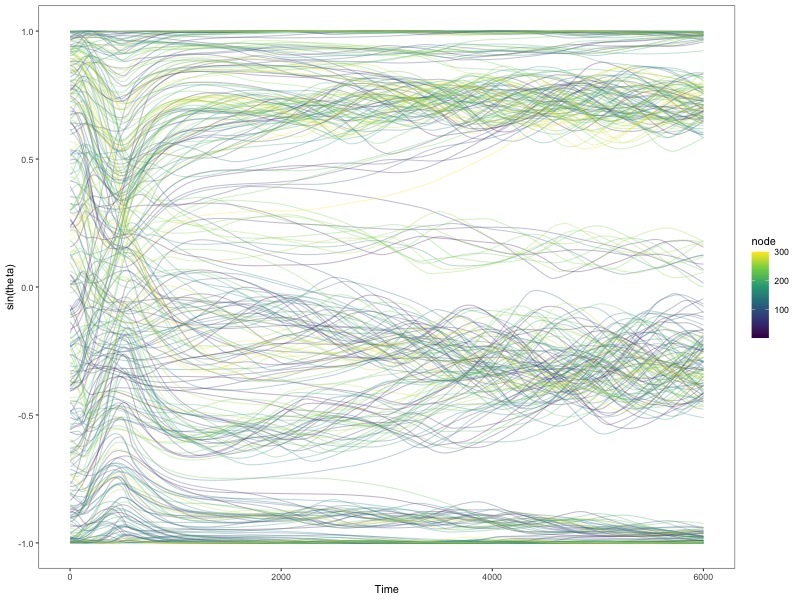
\includegraphics[width=\textwidth]{images/appendix-task1/Splintered_phase_wave.jpg}
        \caption{Splinter phase wave  state\newline
        ($K=-0.1$, $J=1$)}
        \label{fig:splinter_phase_wave_p}
    \end{minipage}
\end{figure}

%###########################
\begin{figure} [p]
   \begin{minipage}{\textwidth}
    \centering
    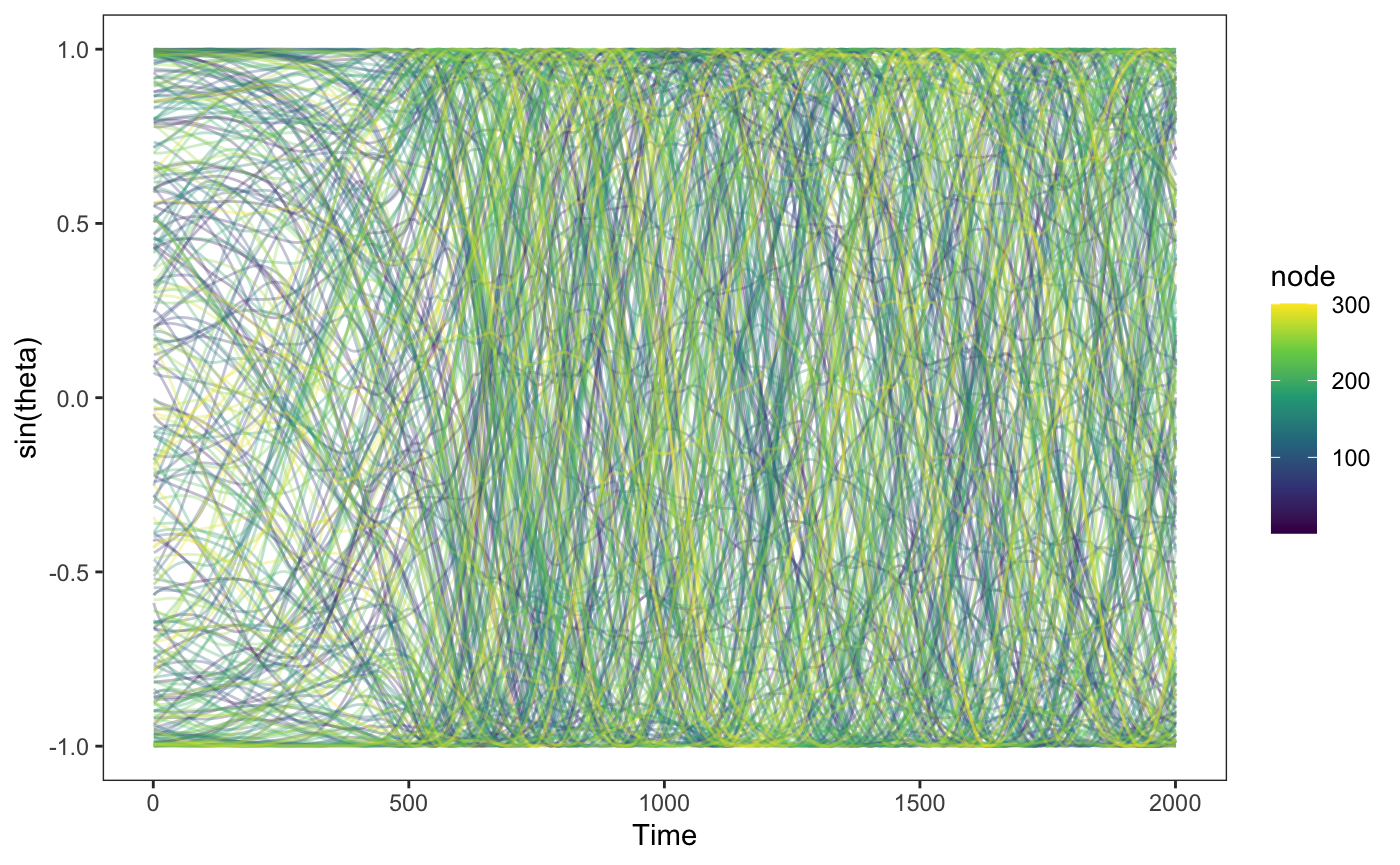
\includegraphics[width=\textwidth]{images/appendix-task1/Active_phase_wave.png}
    \caption{Active phase wave state \\ \parbox[t]{\textwidth}{\raggedright ($K=-0.6$, $J=0.9$)}}
    \label{fig:active_phase_wave_p}
\end{minipage}
\end{figure}